
% Default to the notebook output style

    


% Inherit from the specified cell style.




    
\documentclass[11pt]{article}

    
    
    \usepackage[T1]{fontenc}
    % Nicer default font (+ math font) than Computer Modern for most use cases
    \usepackage{mathpazo}

    % Basic figure setup, for now with no caption control since it's done
    % automatically by Pandoc (which extracts ![](path) syntax from Markdown).
    \usepackage{graphicx}
    % We will generate all images so they have a width \maxwidth. This means
    % that they will get their normal width if they fit onto the page, but
    % are scaled down if they would overflow the margins.
    \makeatletter
    \def\maxwidth{\ifdim\Gin@nat@width>\linewidth\linewidth
    \else\Gin@nat@width\fi}
    \makeatother
    \let\Oldincludegraphics\includegraphics
    % Set max figure width to be 80% of text width, for now hardcoded.
    \renewcommand{\includegraphics}[1]{\Oldincludegraphics[width=.8\maxwidth]{#1}}
    % Ensure that by default, figures have no caption (until we provide a
    % proper Figure object with a Caption API and a way to capture that
    % in the conversion process - todo).
    \usepackage{caption}
    \DeclareCaptionLabelFormat{nolabel}{}
    \captionsetup{labelformat=nolabel}

    \usepackage{adjustbox} % Used to constrain images to a maximum size 
    \usepackage{xcolor} % Allow colors to be defined
    \usepackage{enumerate} % Needed for markdown enumerations to work
    \usepackage{geometry} % Used to adjust the document margins
    \usepackage{amsmath} % Equations
    \usepackage{amssymb} % Equations
    \usepackage{textcomp} % defines textquotesingle
    % Hack from http://tex.stackexchange.com/a/47451/13684:
    \AtBeginDocument{%
        \def\PYZsq{\textquotesingle}% Upright quotes in Pygmentized code
    }
    \usepackage{upquote} % Upright quotes for verbatim code
    \usepackage{eurosym} % defines \euro
    \usepackage[mathletters]{ucs} % Extended unicode (utf-8) support
    \usepackage[utf8x]{inputenc} % Allow utf-8 characters in the tex document
    \usepackage{fancyvrb} % verbatim replacement that allows latex
    \usepackage{grffile} % extends the file name processing of package graphics 
                         % to support a larger range 
    % The hyperref package gives us a pdf with properly built
    % internal navigation ('pdf bookmarks' for the table of contents,
    % internal cross-reference links, web links for URLs, etc.)
    \usepackage{hyperref}
    \usepackage{longtable} % longtable support required by pandoc >1.10
    \usepackage{booktabs}  % table support for pandoc > 1.12.2
    \usepackage[inline]{enumitem} % IRkernel/repr support (it uses the enumerate* environment)
    \usepackage[normalem]{ulem} % ulem is needed to support strikethroughs (\sout)
                                % normalem makes italics be italics, not underlines
    

    
    
    % Colors for the hyperref package
    \definecolor{urlcolor}{rgb}{0,.145,.698}
    \definecolor{linkcolor}{rgb}{.71,0.21,0.01}
    \definecolor{citecolor}{rgb}{.12,.54,.11}

    % ANSI colors
    \definecolor{ansi-black}{HTML}{3E424D}
    \definecolor{ansi-black-intense}{HTML}{282C36}
    \definecolor{ansi-red}{HTML}{E75C58}
    \definecolor{ansi-red-intense}{HTML}{B22B31}
    \definecolor{ansi-green}{HTML}{00A250}
    \definecolor{ansi-green-intense}{HTML}{007427}
    \definecolor{ansi-yellow}{HTML}{DDB62B}
    \definecolor{ansi-yellow-intense}{HTML}{B27D12}
    \definecolor{ansi-blue}{HTML}{208FFB}
    \definecolor{ansi-blue-intense}{HTML}{0065CA}
    \definecolor{ansi-magenta}{HTML}{D160C4}
    \definecolor{ansi-magenta-intense}{HTML}{A03196}
    \definecolor{ansi-cyan}{HTML}{60C6C8}
    \definecolor{ansi-cyan-intense}{HTML}{258F8F}
    \definecolor{ansi-white}{HTML}{C5C1B4}
    \definecolor{ansi-white-intense}{HTML}{A1A6B2}

    % commands and environments needed by pandoc snippets
    % extracted from the output of `pandoc -s`
    \providecommand{\tightlist}{%
      \setlength{\itemsep}{0pt}\setlength{\parskip}{0pt}}
    \DefineVerbatimEnvironment{Highlighting}{Verbatim}{commandchars=\\\{\}}
    % Add ',fontsize=\small' for more characters per line
    \newenvironment{Shaded}{}{}
    \newcommand{\KeywordTok}[1]{\textcolor[rgb]{0.00,0.44,0.13}{\textbf{{#1}}}}
    \newcommand{\DataTypeTok}[1]{\textcolor[rgb]{0.56,0.13,0.00}{{#1}}}
    \newcommand{\DecValTok}[1]{\textcolor[rgb]{0.25,0.63,0.44}{{#1}}}
    \newcommand{\BaseNTok}[1]{\textcolor[rgb]{0.25,0.63,0.44}{{#1}}}
    \newcommand{\FloatTok}[1]{\textcolor[rgb]{0.25,0.63,0.44}{{#1}}}
    \newcommand{\CharTok}[1]{\textcolor[rgb]{0.25,0.44,0.63}{{#1}}}
    \newcommand{\StringTok}[1]{\textcolor[rgb]{0.25,0.44,0.63}{{#1}}}
    \newcommand{\CommentTok}[1]{\textcolor[rgb]{0.38,0.63,0.69}{\textit{{#1}}}}
    \newcommand{\OtherTok}[1]{\textcolor[rgb]{0.00,0.44,0.13}{{#1}}}
    \newcommand{\AlertTok}[1]{\textcolor[rgb]{1.00,0.00,0.00}{\textbf{{#1}}}}
    \newcommand{\FunctionTok}[1]{\textcolor[rgb]{0.02,0.16,0.49}{{#1}}}
    \newcommand{\RegionMarkerTok}[1]{{#1}}
    \newcommand{\ErrorTok}[1]{\textcolor[rgb]{1.00,0.00,0.00}{\textbf{{#1}}}}
    \newcommand{\NormalTok}[1]{{#1}}
    
    % Additional commands for more recent versions of Pandoc
    \newcommand{\ConstantTok}[1]{\textcolor[rgb]{0.53,0.00,0.00}{{#1}}}
    \newcommand{\SpecialCharTok}[1]{\textcolor[rgb]{0.25,0.44,0.63}{{#1}}}
    \newcommand{\VerbatimStringTok}[1]{\textcolor[rgb]{0.25,0.44,0.63}{{#1}}}
    \newcommand{\SpecialStringTok}[1]{\textcolor[rgb]{0.73,0.40,0.53}{{#1}}}
    \newcommand{\ImportTok}[1]{{#1}}
    \newcommand{\DocumentationTok}[1]{\textcolor[rgb]{0.73,0.13,0.13}{\textit{{#1}}}}
    \newcommand{\AnnotationTok}[1]{\textcolor[rgb]{0.38,0.63,0.69}{\textbf{\textit{{#1}}}}}
    \newcommand{\CommentVarTok}[1]{\textcolor[rgb]{0.38,0.63,0.69}{\textbf{\textit{{#1}}}}}
    \newcommand{\VariableTok}[1]{\textcolor[rgb]{0.10,0.09,0.49}{{#1}}}
    \newcommand{\ControlFlowTok}[1]{\textcolor[rgb]{0.00,0.44,0.13}{\textbf{{#1}}}}
    \newcommand{\OperatorTok}[1]{\textcolor[rgb]{0.40,0.40,0.40}{{#1}}}
    \newcommand{\BuiltInTok}[1]{{#1}}
    \newcommand{\ExtensionTok}[1]{{#1}}
    \newcommand{\PreprocessorTok}[1]{\textcolor[rgb]{0.74,0.48,0.00}{{#1}}}
    \newcommand{\AttributeTok}[1]{\textcolor[rgb]{0.49,0.56,0.16}{{#1}}}
    \newcommand{\InformationTok}[1]{\textcolor[rgb]{0.38,0.63,0.69}{\textbf{\textit{{#1}}}}}
    \newcommand{\WarningTok}[1]{\textcolor[rgb]{0.38,0.63,0.69}{\textbf{\textit{{#1}}}}}
    
    
    % Define a nice break command that doesn't care if a line doesn't already
    % exist.
    \def\br{\hspace*{\fill} \\* }
    % Math Jax compatability definitions
    \def\gt{>}
    \def\lt{<}
    % Document parameters
    \title{ECCO\_v4\_data\_structure\_basics}
    
    
    

    % Pygments definitions
    
\makeatletter
\def\PY@reset{\let\PY@it=\relax \let\PY@bf=\relax%
    \let\PY@ul=\relax \let\PY@tc=\relax%
    \let\PY@bc=\relax \let\PY@ff=\relax}
\def\PY@tok#1{\csname PY@tok@#1\endcsname}
\def\PY@toks#1+{\ifx\relax#1\empty\else%
    \PY@tok{#1}\expandafter\PY@toks\fi}
\def\PY@do#1{\PY@bc{\PY@tc{\PY@ul{%
    \PY@it{\PY@bf{\PY@ff{#1}}}}}}}
\def\PY#1#2{\PY@reset\PY@toks#1+\relax+\PY@do{#2}}

\expandafter\def\csname PY@tok@gd\endcsname{\def\PY@tc##1{\textcolor[rgb]{0.63,0.00,0.00}{##1}}}
\expandafter\def\csname PY@tok@gu\endcsname{\let\PY@bf=\textbf\def\PY@tc##1{\textcolor[rgb]{0.50,0.00,0.50}{##1}}}
\expandafter\def\csname PY@tok@gt\endcsname{\def\PY@tc##1{\textcolor[rgb]{0.00,0.27,0.87}{##1}}}
\expandafter\def\csname PY@tok@gs\endcsname{\let\PY@bf=\textbf}
\expandafter\def\csname PY@tok@gr\endcsname{\def\PY@tc##1{\textcolor[rgb]{1.00,0.00,0.00}{##1}}}
\expandafter\def\csname PY@tok@cm\endcsname{\let\PY@it=\textit\def\PY@tc##1{\textcolor[rgb]{0.25,0.50,0.50}{##1}}}
\expandafter\def\csname PY@tok@vg\endcsname{\def\PY@tc##1{\textcolor[rgb]{0.10,0.09,0.49}{##1}}}
\expandafter\def\csname PY@tok@vi\endcsname{\def\PY@tc##1{\textcolor[rgb]{0.10,0.09,0.49}{##1}}}
\expandafter\def\csname PY@tok@vm\endcsname{\def\PY@tc##1{\textcolor[rgb]{0.10,0.09,0.49}{##1}}}
\expandafter\def\csname PY@tok@mh\endcsname{\def\PY@tc##1{\textcolor[rgb]{0.40,0.40,0.40}{##1}}}
\expandafter\def\csname PY@tok@cs\endcsname{\let\PY@it=\textit\def\PY@tc##1{\textcolor[rgb]{0.25,0.50,0.50}{##1}}}
\expandafter\def\csname PY@tok@ge\endcsname{\let\PY@it=\textit}
\expandafter\def\csname PY@tok@vc\endcsname{\def\PY@tc##1{\textcolor[rgb]{0.10,0.09,0.49}{##1}}}
\expandafter\def\csname PY@tok@il\endcsname{\def\PY@tc##1{\textcolor[rgb]{0.40,0.40,0.40}{##1}}}
\expandafter\def\csname PY@tok@go\endcsname{\def\PY@tc##1{\textcolor[rgb]{0.53,0.53,0.53}{##1}}}
\expandafter\def\csname PY@tok@cp\endcsname{\def\PY@tc##1{\textcolor[rgb]{0.74,0.48,0.00}{##1}}}
\expandafter\def\csname PY@tok@gi\endcsname{\def\PY@tc##1{\textcolor[rgb]{0.00,0.63,0.00}{##1}}}
\expandafter\def\csname PY@tok@gh\endcsname{\let\PY@bf=\textbf\def\PY@tc##1{\textcolor[rgb]{0.00,0.00,0.50}{##1}}}
\expandafter\def\csname PY@tok@ni\endcsname{\let\PY@bf=\textbf\def\PY@tc##1{\textcolor[rgb]{0.60,0.60,0.60}{##1}}}
\expandafter\def\csname PY@tok@nl\endcsname{\def\PY@tc##1{\textcolor[rgb]{0.63,0.63,0.00}{##1}}}
\expandafter\def\csname PY@tok@nn\endcsname{\let\PY@bf=\textbf\def\PY@tc##1{\textcolor[rgb]{0.00,0.00,1.00}{##1}}}
\expandafter\def\csname PY@tok@no\endcsname{\def\PY@tc##1{\textcolor[rgb]{0.53,0.00,0.00}{##1}}}
\expandafter\def\csname PY@tok@na\endcsname{\def\PY@tc##1{\textcolor[rgb]{0.49,0.56,0.16}{##1}}}
\expandafter\def\csname PY@tok@nb\endcsname{\def\PY@tc##1{\textcolor[rgb]{0.00,0.50,0.00}{##1}}}
\expandafter\def\csname PY@tok@nc\endcsname{\let\PY@bf=\textbf\def\PY@tc##1{\textcolor[rgb]{0.00,0.00,1.00}{##1}}}
\expandafter\def\csname PY@tok@nd\endcsname{\def\PY@tc##1{\textcolor[rgb]{0.67,0.13,1.00}{##1}}}
\expandafter\def\csname PY@tok@ne\endcsname{\let\PY@bf=\textbf\def\PY@tc##1{\textcolor[rgb]{0.82,0.25,0.23}{##1}}}
\expandafter\def\csname PY@tok@nf\endcsname{\def\PY@tc##1{\textcolor[rgb]{0.00,0.00,1.00}{##1}}}
\expandafter\def\csname PY@tok@si\endcsname{\let\PY@bf=\textbf\def\PY@tc##1{\textcolor[rgb]{0.73,0.40,0.53}{##1}}}
\expandafter\def\csname PY@tok@s2\endcsname{\def\PY@tc##1{\textcolor[rgb]{0.73,0.13,0.13}{##1}}}
\expandafter\def\csname PY@tok@nt\endcsname{\let\PY@bf=\textbf\def\PY@tc##1{\textcolor[rgb]{0.00,0.50,0.00}{##1}}}
\expandafter\def\csname PY@tok@nv\endcsname{\def\PY@tc##1{\textcolor[rgb]{0.10,0.09,0.49}{##1}}}
\expandafter\def\csname PY@tok@s1\endcsname{\def\PY@tc##1{\textcolor[rgb]{0.73,0.13,0.13}{##1}}}
\expandafter\def\csname PY@tok@dl\endcsname{\def\PY@tc##1{\textcolor[rgb]{0.73,0.13,0.13}{##1}}}
\expandafter\def\csname PY@tok@ch\endcsname{\let\PY@it=\textit\def\PY@tc##1{\textcolor[rgb]{0.25,0.50,0.50}{##1}}}
\expandafter\def\csname PY@tok@m\endcsname{\def\PY@tc##1{\textcolor[rgb]{0.40,0.40,0.40}{##1}}}
\expandafter\def\csname PY@tok@gp\endcsname{\let\PY@bf=\textbf\def\PY@tc##1{\textcolor[rgb]{0.00,0.00,0.50}{##1}}}
\expandafter\def\csname PY@tok@sh\endcsname{\def\PY@tc##1{\textcolor[rgb]{0.73,0.13,0.13}{##1}}}
\expandafter\def\csname PY@tok@ow\endcsname{\let\PY@bf=\textbf\def\PY@tc##1{\textcolor[rgb]{0.67,0.13,1.00}{##1}}}
\expandafter\def\csname PY@tok@sx\endcsname{\def\PY@tc##1{\textcolor[rgb]{0.00,0.50,0.00}{##1}}}
\expandafter\def\csname PY@tok@bp\endcsname{\def\PY@tc##1{\textcolor[rgb]{0.00,0.50,0.00}{##1}}}
\expandafter\def\csname PY@tok@c1\endcsname{\let\PY@it=\textit\def\PY@tc##1{\textcolor[rgb]{0.25,0.50,0.50}{##1}}}
\expandafter\def\csname PY@tok@fm\endcsname{\def\PY@tc##1{\textcolor[rgb]{0.00,0.00,1.00}{##1}}}
\expandafter\def\csname PY@tok@o\endcsname{\def\PY@tc##1{\textcolor[rgb]{0.40,0.40,0.40}{##1}}}
\expandafter\def\csname PY@tok@kc\endcsname{\let\PY@bf=\textbf\def\PY@tc##1{\textcolor[rgb]{0.00,0.50,0.00}{##1}}}
\expandafter\def\csname PY@tok@c\endcsname{\let\PY@it=\textit\def\PY@tc##1{\textcolor[rgb]{0.25,0.50,0.50}{##1}}}
\expandafter\def\csname PY@tok@mf\endcsname{\def\PY@tc##1{\textcolor[rgb]{0.40,0.40,0.40}{##1}}}
\expandafter\def\csname PY@tok@err\endcsname{\def\PY@bc##1{\setlength{\fboxsep}{0pt}\fcolorbox[rgb]{1.00,0.00,0.00}{1,1,1}{\strut ##1}}}
\expandafter\def\csname PY@tok@mb\endcsname{\def\PY@tc##1{\textcolor[rgb]{0.40,0.40,0.40}{##1}}}
\expandafter\def\csname PY@tok@ss\endcsname{\def\PY@tc##1{\textcolor[rgb]{0.10,0.09,0.49}{##1}}}
\expandafter\def\csname PY@tok@sr\endcsname{\def\PY@tc##1{\textcolor[rgb]{0.73,0.40,0.53}{##1}}}
\expandafter\def\csname PY@tok@mo\endcsname{\def\PY@tc##1{\textcolor[rgb]{0.40,0.40,0.40}{##1}}}
\expandafter\def\csname PY@tok@kd\endcsname{\let\PY@bf=\textbf\def\PY@tc##1{\textcolor[rgb]{0.00,0.50,0.00}{##1}}}
\expandafter\def\csname PY@tok@mi\endcsname{\def\PY@tc##1{\textcolor[rgb]{0.40,0.40,0.40}{##1}}}
\expandafter\def\csname PY@tok@kn\endcsname{\let\PY@bf=\textbf\def\PY@tc##1{\textcolor[rgb]{0.00,0.50,0.00}{##1}}}
\expandafter\def\csname PY@tok@cpf\endcsname{\let\PY@it=\textit\def\PY@tc##1{\textcolor[rgb]{0.25,0.50,0.50}{##1}}}
\expandafter\def\csname PY@tok@kr\endcsname{\let\PY@bf=\textbf\def\PY@tc##1{\textcolor[rgb]{0.00,0.50,0.00}{##1}}}
\expandafter\def\csname PY@tok@s\endcsname{\def\PY@tc##1{\textcolor[rgb]{0.73,0.13,0.13}{##1}}}
\expandafter\def\csname PY@tok@kp\endcsname{\def\PY@tc##1{\textcolor[rgb]{0.00,0.50,0.00}{##1}}}
\expandafter\def\csname PY@tok@w\endcsname{\def\PY@tc##1{\textcolor[rgb]{0.73,0.73,0.73}{##1}}}
\expandafter\def\csname PY@tok@kt\endcsname{\def\PY@tc##1{\textcolor[rgb]{0.69,0.00,0.25}{##1}}}
\expandafter\def\csname PY@tok@sc\endcsname{\def\PY@tc##1{\textcolor[rgb]{0.73,0.13,0.13}{##1}}}
\expandafter\def\csname PY@tok@sb\endcsname{\def\PY@tc##1{\textcolor[rgb]{0.73,0.13,0.13}{##1}}}
\expandafter\def\csname PY@tok@sa\endcsname{\def\PY@tc##1{\textcolor[rgb]{0.73,0.13,0.13}{##1}}}
\expandafter\def\csname PY@tok@k\endcsname{\let\PY@bf=\textbf\def\PY@tc##1{\textcolor[rgb]{0.00,0.50,0.00}{##1}}}
\expandafter\def\csname PY@tok@se\endcsname{\let\PY@bf=\textbf\def\PY@tc##1{\textcolor[rgb]{0.73,0.40,0.13}{##1}}}
\expandafter\def\csname PY@tok@sd\endcsname{\let\PY@it=\textit\def\PY@tc##1{\textcolor[rgb]{0.73,0.13,0.13}{##1}}}

\def\PYZbs{\char`\\}
\def\PYZus{\char`\_}
\def\PYZob{\char`\{}
\def\PYZcb{\char`\}}
\def\PYZca{\char`\^}
\def\PYZam{\char`\&}
\def\PYZlt{\char`\<}
\def\PYZgt{\char`\>}
\def\PYZsh{\char`\#}
\def\PYZpc{\char`\%}
\def\PYZdl{\char`\$}
\def\PYZhy{\char`\-}
\def\PYZsq{\char`\'}
\def\PYZdq{\char`\"}
\def\PYZti{\char`\~}
% for compatibility with earlier versions
\def\PYZat{@}
\def\PYZlb{[}
\def\PYZrb{]}
\makeatother


    % Exact colors from NB
    \definecolor{incolor}{rgb}{0.0, 0.0, 0.5}
    \definecolor{outcolor}{rgb}{0.545, 0.0, 0.0}



    
    % Prevent overflowing lines due to hard-to-break entities
    \sloppy 
    % Setup hyperref package
    \hypersetup{
      breaklinks=true,  % so long urls are correctly broken across lines
      colorlinks=true,
      urlcolor=urlcolor,
      linkcolor=linkcolor,
      citecolor=citecolor,
      }
    % Slightly bigger margins than the latex defaults
    
    \geometry{verbose,tmargin=1in,bmargin=1in,lmargin=1in,rmargin=1in}
    
    

    \begin{document}
    
    
    \maketitle
    
    

    
    \section{The Dataset and DataArray Objects Used in the ECCOv4 Python
Package.}\label{the-dataset-and-dataarray-objects-used-in-the-eccov4-python-package.}

\subsection{Objectives:}\label{objectives}

To introduce the two high-level data structures, \texttt{Dataset} and
\texttt{DataArray}, that are used in by the ECCOv4 Python package to
load and store the ECCO model grid parameters and state estimate
variables

Because this is the first tutorial, we describe every step in detail.
Later tutorials will be less explicit about describing the basic
operations required to begin working with the state estimate.

Let's get started.

\subsection{Import external packages and
modules}\label{import-external-packages-and-modules}

At the beginning of every Python program or interactive instance we need
to import helpful non-core modules or packages. Modules or packages that
are loaded into the environment can be thought of as external code
libraries and contain subroutines and/or data objects that provide
useful functionality.

    \begin{Verbatim}[commandchars=\\\{\}]
{\color{incolor}In [{\color{incolor}1}]:} \PY{c+c1}{\PYZsh{} Matplotlib is a Python 2D plotting library which produces publication quality}
        \PY{c+c1}{\PYZsh{} figures in a variety of hardcopy formats and interactive environments across }
        \PY{c+c1}{\PYZsh{} platforms.}
        \PY{c+c1}{\PYZsh{} https://matplotlib.org/}
        \PY{c+c1}{\PYZsh{}}
        \PY{c+c1}{\PYZsh{} make all functions from the \PYZsq{}matplotlib.pylab\PYZsq{} module available with the }
        \PY{c+c1}{\PYZsh{} prefix \PYZsq{}plt\PYZsq{}}
        \PY{k+kn}{import} \PY{n+nn}{matplotlib.pylab} \PY{k+kn}{as} \PY{n+nn}{plt}
        
        \PY{c+c1}{\PYZsh{} NumPy is the fundamental package for scientific computing with Python. }
        \PY{c+c1}{\PYZsh{} It contains among other things:}
        \PY{c+c1}{\PYZsh{}    a powerful N\PYZhy{}dimensional array object}
        \PY{c+c1}{\PYZsh{}    sophisticated (broadcasting) functions}
        \PY{c+c1}{\PYZsh{}    tools for integrating C/C++ and Fortran code}
        \PY{c+c1}{\PYZsh{}    useful linear algebra, Fourier transform, and random number capabilities}
        \PY{c+c1}{\PYZsh{} http://www.numpy.org/}
        \PY{c+c1}{\PYZsh{}}
        \PY{c+c1}{\PYZsh{} make all functions from the \PYZsq{}numpy\PYZsq{} module available with the prefix \PYZsq{}np\PYZsq{}}
        \PY{k+kn}{import} \PY{n+nn}{numpy} \PY{k+kn}{as} \PY{n+nn}{np}
        
        \PY{c+c1}{\PYZsh{} make all functions from the \PYZsq{}sys\PYZsq{} module available with the prefix \PYZsq{}sys\PYZsq{}}
        \PY{k+kn}{import} \PY{n+nn}{sys}
        
        \PY{c+c1}{\PYZsh{} xarray is an open source project and Python package that aims to bring the }
        \PY{c+c1}{\PYZsh{} labeled data power of pandas to the physical sciences, by providing}
        \PY{c+c1}{\PYZsh{} N\PYZhy{}dimensional variants of the core pandas data structures.}
        \PY{c+c1}{\PYZsh{} Our approach adopts the Common Data Model for self\PYZhy{} describing scientific }
        \PY{c+c1}{\PYZsh{} data in widespread use in the Earth sciences: xarray.Dataset is an in\PYZhy{}memory}
        \PY{c+c1}{\PYZsh{} representation of a netCDF file.}
        \PY{c+c1}{\PYZsh{} http://xarray.pydata.org/en/stable/}
        \PY{c+c1}{\PYZsh{}}
        \PY{c+c1}{\PYZsh{} import all function from the \PYZsq{}xarray\PYZsq{} module available with the prefix \PYZsq{}xr\PYZsq{}}
        \PY{k+kn}{import} \PY{n+nn}{xarray} \PY{k+kn}{as} \PY{n+nn}{xr}
        
        \PY{c+c1}{\PYZsh{} The matplotlib basemap toolkit is a library for plotting 2D data on maps in}
        \PY{c+c1}{\PYZsh{} Python. ... Basemap is geared toward the needs of earth scientists, }
        \PY{c+c1}{\PYZsh{} particularly oceanographers and meteorologists. }
        \PY{c+c1}{\PYZsh{} https://matplotlib.org/basemap/index.html}
        \PY{c+c1}{\PYZsh{}}
        \PY{c+c1}{\PYZsh{} The \PYZsq{}copy\PYZsq{} module provides generic ... copy operations.\PYZdq{}}
        \PY{c+c1}{\PYZsh{} \PYZdq{}Assignment statements in Python do not copy objects, they create }
        \PY{c+c1}{\PYZsh{} bindings [pointers] between a target and an object.\PYZdq{} \PYZdq{}... a copy is }
        \PY{c+c1}{\PYZsh{} sometimes needed so one can change one copy without changing the other.\PYZdq{}}
        \PY{c+c1}{\PYZsh{} https://docs.python.org/2/library/copy.html}
        \PY{c+c1}{\PYZsh{}}
        \PY{c+c1}{\PYZsh{} import the \PYZsq{}deepcopy\PYZsq{} function from the \PYZsq{}copy\PYZsq{} module}
        \PY{k+kn}{from} \PY{n+nn}{copy} \PY{k+kn}{import} \PY{n}{deepcopy} 
        
        \PY{c+c1}{\PYZsh{} Modules to display images in Jupyter notebooks:}
        \PY{k+kn}{from} \PY{n+nn}{IPython.display} \PY{k+kn}{import} \PY{n}{Image}
        \PY{k+kn}{from} \PY{n+nn}{IPython.core.display} \PY{k+kn}{import} \PY{n}{HTML} 
\end{Verbatim}


    \subsubsection{Load the ECCO Version 4 Python
package}\label{load-the-ecco-version-4-python-package}

The \emph{ecco\_v4\_py} is a Python package written specifically for
working with the netcdf output provided in the
\href{ftp://ecco.jpl.nasa.gov/Version4/Release3/nctiles_monthly/}{nctiles\_monthly}
directory of the \href{ftp://ecco.jpl.nasa.gov/Version4/Release3/}{ECCO
v4 release}

See the "Getting Started" page in the tutorial for instructions about
installing the \emph{ecco\_v4\_py} module on your machine.

    \begin{Verbatim}[commandchars=\\\{\}]
{\color{incolor}In [{\color{incolor}2}]:} \PY{k+kn}{import} \PY{n+nn}{ecco\PYZus{}v4\PYZus{}py} \PY{k+kn}{as} \PY{n+nn}{ecco}
\end{Verbatim}


    The syntax \emph{import X package as Y} allows you to access all of the
subroutines and other objects in X by typing
\emph{Y.some\_routine\_in\_X}. Here, we import \texttt{ecco\_v4\_py} as
\texttt{ecco} because it is less to type than \emph{ecco\_v4\_py} and by
doing so we can access many subroutines spread out over several modules
within the \emph{ecco\_v4\_py} package.

    \subsection{Load a single netCDF grid tile
file}\label{load-a-single-netcdf-grid-tile-file}

To load ECCO v4's netcdf files we will use the \emph{open\_dataset}
command from the
\href{http://xarray.pydata.org/en/stable/index.html}{xarray} Python
package. \emph{open\_dataset} creates a \textbf{Dataset} object and
loads the contents of the netcdf file, including its metadata, into a
data structure.

Let's open the grid file for \emph{tile 3} (North East Atlantic Ocean),
of the 13 ECCO v4 llc90 grid files.

Change \texttt{data\_dir} to match the location of your
\texttt{nctiles\_grid} directory.

    \begin{Verbatim}[commandchars=\\\{\}]
{\color{incolor}In [{\color{incolor}3}]:} \PY{n}{grid\PYZus{}dir}\PY{o}{=}\PY{l+s+s1}{\PYZsq{}}\PY{l+s+s1}{/Volumes/ECCO\PYZus{}BASE/ECCO\PYZus{}v4r3/nctiles\PYZus{}grid/}\PY{l+s+s1}{\PYZsq{}}    
        
        \PY{n}{fname} \PY{o}{=} \PY{l+s+s1}{\PYZsq{}}\PY{l+s+s1}{GRID.0003.nc}\PY{l+s+s1}{\PYZsq{}}
        \PY{n}{ds} \PY{o}{=} \PY{n}{xr}\PY{o}{.}\PY{n}{open\PYZus{}dataset}\PY{p}{(}\PY{n}{grid\PYZus{}dir} \PY{o}{+} \PY{n}{fname}\PY{p}{)}
\end{Verbatim}


    \begin{Verbatim}[commandchars=\\\{\}]
{\color{incolor}In [{\color{incolor}4}]:} \PY{n+nb}{type}\PY{p}{(}\PY{n}{ds}\PY{p}{)}
\end{Verbatim}


\begin{Verbatim}[commandchars=\\\{\}]
{\color{outcolor}Out[{\color{outcolor}4}]:} xarray.core.dataset.Dataset
\end{Verbatim}
            
    \subsection{The Dataset object}\label{the-dataset-object}

According to the xarray documentation, a
\href{http://xarray.pydata.org/en/stable/generated/xarray.Dataset.html}{Dataset}
is a "Python object designed as an "in-memory representation of the data
model from the netCDF file format."

What does that mean? netCDF files are \emph{self-describing} in the
sense that they
\href{https://www.unidata.ucar.edu/software/netcdf/docs/faq.html}{include
information about the data they contain}. When Dataset objects are
created by loading a netCDF file they contain all of the same data and
metadata provided by the netCDF file.

Just as a netCDF file can contain many variables, a \texttt{Dataset}
object can contain many variables. These variables are referred to as
\texttt{Data\ Variables} in the \texttt{xarray} nomenclature.

Dataset objects contain three main classes of fields:

\begin{enumerate}
\def\labelenumi{\arabic{enumi}.}
\tightlist
\item
  \textbf{Coordinates} : indices and labels for all of the coordinates
  used by all data variables
\item
  \textbf{Data Variables}: \texttt{DataArray} objects which contain
  numerical arrays, their coordinates, coordinate labels, and
  variable-specific metadata
\item
  \textbf{Attributes} : metadata
\end{enumerate}

Now that we've loaded \texttt{GRID.0003.nc} into the \texttt{ds}
\texttt{Dataset} object, let's examine its contents.

\begin{quote}
\textbf{Note:} \emph{You can get information about objects and their
contents by typing the name of the variable and hitting \textbf{enter}
in an interactive session of an IDE such as Spyder or a Jupyter
notebook.}
\end{quote}

    \begin{Verbatim}[commandchars=\\\{\}]
{\color{incolor}In [{\color{incolor}5}]:} \PY{n}{ds}
\end{Verbatim}


\begin{Verbatim}[commandchars=\\\{\}]
{\color{outcolor}Out[{\color{outcolor}5}]:} <xarray.Dataset>
        Dimensions:  (i1: 50, i2: 90, i3: 90)
        Coordinates:
          * i1       (i1) float64 1.0 2.0 3.0 4.0 5.0 6.0 7.0 8.0 9.0 10.0 11.0 12.0 {\ldots}
          * i2       (i2) float64 1.0 2.0 3.0 4.0 5.0 6.0 7.0 8.0 9.0 10.0 11.0 12.0 {\ldots}
          * i3       (i3) float64 1.0 2.0 3.0 4.0 5.0 6.0 7.0 8.0 9.0 10.0 11.0 12.0 {\ldots}
        Data variables:
            hFacC    (i1, i2, i3) float64 {\ldots}
            hFacW    (i1, i2, i3) float64 {\ldots}
            hFacS    (i1, i2, i3) float64 {\ldots}
            XC       (i2, i3) float64 {\ldots}
            YC       (i2, i3) float64 {\ldots}
            XG       (i2, i3) float64 {\ldots}
            YG       (i2, i3) float64 {\ldots}
            RAC      (i2, i3) float64 {\ldots}
            RAZ      (i2, i3) float64 {\ldots}
            DXC      (i2, i3) float64 {\ldots}
            DYC      (i2, i3) float64 {\ldots}
            DXG      (i2, i3) float64 {\ldots}
            DYG      (i2, i3) float64 {\ldots}
            Depth    (i2, i3) float64 {\ldots}
            AngleCS  (i2, i3) float64 {\ldots}
            AngleSN  (i2, i3) float64 {\ldots}
            RC       (i1) float64 {\ldots}
            RF       (i1) float64 {\ldots}
            DRC      (i1) float64 {\ldots}
            DRF      (i1) float64 {\ldots}
        Attributes:
            description:    C-grid parameters (see MITgcm documentation for details){\ldots}
            A:              :Format      = native grid (nctiles w. 13 tiles)
            B:              :source      = ECCO consortium (http://ecco-group.org/)
            C:              :institution = JPL/UT/MIT/AER
            D:              :history     = files revision history :
            E:                                 04/20/2017: fill in geometry info for {\ldots}
            F:                                 11/06/2016: third release of ECCO v4 ({\ldots}
            G:                             estimates revision history (from second re{\ldots}
            H:                                 employs bi-harmonic viscosity (enhance{\ldots}
            I:                                 sea-ice parameters, updated or novel o{\ldots}
            J:                                 GRACE OBP, Aquarius SSS, global mean s{\ldots}
            K:                                 time-series, extended and/or expanded {\ldots}
            L:                                 revised weights including data and con{\ldots}
            M:                                 to account for grid-size variation and{\ldots}
            N:                                 separate time-mean and time-variable d{\ldots}
            O:                                 and controls, sea-ice costs, and initi{\ldots}
            P:                                 additional controls.\textbackslash{}n 
            Q:              :references  = Forget, G., J.-M. Campin, P. Heimbach, C. {\ldots}
            R:                              and C. Wunsch, 2015: ECCO version 4: an i{\ldots}
            S:                              non-linear inverse modeling and global oc{\ldots}
            T:                              Geoscientific Model Development, 8, 3071-{\ldots}
            U:                             Forget, G., J.-M. Campin, P. Heimbach, C. {\ldots}
            V:                              ECCO version 4: Second Release, 2016, htt{\ldots}
            W:              file created using gcmfaces\_IO/write2nctiles.m
            date:           21-Apr-2017
            Conventions:    CF-1.6
            \_FillValue:     nan
            missing\_value:  nan
\end{Verbatim}
            
    \subsubsection{Examining the Dataset object
contents}\label{examining-the-dataset-object-contents}

Let's go through \texttt{ds} piece by piece, starting from the top.

\paragraph{1. Object type}\label{object-type}

\texttt{\textless{}xarray.Dataset\textgreater{}}

The top line tells us what type of object the variable is. In this case
\texttt{ds} is an instance of the \texttt{Dataset} object from the
\texttt{xarray} package.

\paragraph{2. Dimensions}\label{dimensions}

\texttt{Dimensions:\ \ (i1:\ 50,\ i2:\ 90,\ i3:\ 90)}

The \emph{Dimensions} list shows all of the different dimensions used by
all of the different arrays stored in the netCDF file (and now loaded in
the \texttt{Dataset} object.)

Arrays may use any combination of these dimensions. In the case of the
netcdf ECCO grid file that we've loaded, there are 1D, 2D, and 3D
arrays.

The names and lengths of the three dimensions is given by:
\texttt{(i1:\ 50,\ i2:\ 90,\ i3:\ 90)}. There are 50 vertical levels in
the ECCO v4 model grid so the \texttt{i1} obviously corresponds to the
vertical dimension while \texttt{i2}\textbar{} and \texttt{i3}
correspond to the horizontal dimensions.

\begin{quote}
\textbf{Note:} Each tile in the llc90 grid used by ECCO v4 has 90x90
horizontal grid points. That's where the "90: in llc\textbf{90} comes
from!
\end{quote}

\paragraph{3. Coordinates}\label{coordinates}

\begin{verbatim}
Coordinates:
    i1       (i1) float64 1.0 2.0 3.0 4.0 5.0 6.0 7.0 8.0 9.0 10.0 11.0 12.0 ...
    i2       (i2) float64 1.0 2.0 3.0 4.0 5.0 6.0 7.0 8.0 9.0 10.0 11.0 12.0 ...
    i3       (i3) float64 1.0 2.0 3.0 4.0 5.0 6.0 7.0 8.0 9.0 10.0 11.0 12.0 ... 
\end{verbatim}

\textbf{i1}, \textbf{i2}, and \textbf{i3} are the
\href{http://xarray.pydata.org/en/stable/data-structures.html\#coordinates}{coordinates},
which are Python dictionaries of arrays whose values \emph{label} each
point. They are used for label-based indexing and alignment.

In this case, the \emph{coordinates} of each dimension consist of
\emph{labels} \([1, 2, ... n]\), where \(n\) is the length of the
dimension:

\begin{itemize}
\tightlist
\item
  Dim \textbf{i1}: \texttt{array({[}\ \ 1.,\ \ \ 2.,\ ...,\ 50.{]})}
\item
  Dim \textbf{i2} and \textbf{i3}:
  \texttt{array({[}\ \ 1.,\ \ \ 2.,\ ...,\ 90.{]})}
\end{itemize}

\begin{quote}
\textbf{Note:} Actually these coordinates are \textbf{Dimension
coordinates} which are one dimensional coordinates (marked by an asterix
\textbf{"*"} when printing a dataset or data array). Don't worry what
that means for now, we'll return to the topic in a later tutorial.
\end{quote}

\paragraph{4. Data Variables}\label{data-variables}

\begin{verbatim}
Data variables:
    hFacC    (i1, i2, i3) float64 ...
    hFacW    (i1, i2, i3) float64 ...
    hFacS    (i1, i2, i3) float64 ...
    ...
    XC       (i2, i3) float64 ...
    YC       (i2, i3) float64 ...
    ...
    RC       (i1) float64 ...
    RF       (i1) float64 ...
\end{verbatim}

The \texttt{Data\ Variables} are one or more \texttt{xarray.DataArray}
objects. \texttt{DataArray} objects are labeled, multi-dimensional
arrays that may also contain metadata (attributes). \texttt{DataArray}
objects are very important to understand because they are container
objects that containing the actual numerical arrays for the different
ECCO variables. We'll investigate these objects in more detail after
finishing with the \texttt{Dataset} object.

A subset of all \texttt{Data\ variables} in \texttt{ds} are shown above
to demonstrate that in this netcdf grid file there are variables with
three different dimension combinations: 3D with dimensions (\textbf{i1},
\textbf{i2}, \textbf{i3}), 2D with dimensions (\textbf{i2},
\textbf{i3}), and 1D with dimensions (\textbf{i1})

Here, the 1D variables only have values in the \textbf{i1} (vertical)
dimension, the 2D variables only have values in the \textbf{i2} and
\textbf{i3} (horizontal) dimensions, and the 3D variables have values in
all three dimensions. All of these variables are of type 64 bit float.

\begin{quote}
\textbf{Note:} All ECCO v4 netcdf grid files include a number of grid
parameters. Of these, 3 are 3D, 13 are 2D, and 4 are 1D. The 3D grid
parameters vary with horizontal location and depth (e.g.,
\textbf{hFacC}, the vertical fraction of a grid cell of the Arakawa-C
grid tracer 'c' point). The 2D grid parameters only vary with horizontal
location and are therefore independent of depth (e.g., \textbf{XC} the
longitude of the tracer 'c' point). The 1D grid parameters only vary
with depth and are therefore independent of horizontal location (e.g.,
\textbf{RF} the height of a tracer 'c' grid cell). The meaning of all
MITgcm grid parameters is described in section
\href{http://mitgcm.org/sealion/online_documents/node47.html}{2.10.5 of
the MITgcm documentation}.
\end{quote}

\paragraph{5. Attributes}\label{attributes}

\begin{verbatim}
Attributes:
    description:    C-grid parameters (see MITgcm documentation for details)....
    A:              :Format      = native grid (nctiles w. 13 tiles)
    B:              :source      = ECCO consortium (http://ecco-group.org/)
    C:              :institution = JPL/UT/MIT/AER
    D:              :history     = files revision history :
    E:                                 04/20/2017: fill in geometry info for ...
    F:                                 11/06/2016: third release of ECCO v4 (...
    ...
    W:              file created using gcmfaces_IO/write2nctiles.m
    date:           21-Apr-2017
    Conventions:    CF-1.6
    _FillValue:     nan
    missing_value:  nan
\end{verbatim}

The \texttt{attrs} variable is a Python
\href{https://www.python-course.eu/dictionaries.php}{dictionary object}
containing metadata or any auxilliary information.

Metadata is presented as a set of dictionary \texttt{key-value} pairs.
Here the \texttt{keys} are \emph{description, A, B, ... missing\_value.}
while the \texttt{values} are the corresponding text and non-text
values.

To see the metadata \texttt{value} associated with the metadata
"Conventions" \texttt{key} we type:

    \begin{Verbatim}[commandchars=\\\{\}]
{\color{incolor}In [{\color{incolor}6}]:} \PY{k}{print} \PY{n}{ds}\PY{o}{.}\PY{n}{attrs}\PY{p}{[}\PY{l+s+s1}{\PYZsq{}}\PY{l+s+s1}{Conventions}\PY{l+s+s1}{\PYZsq{}}\PY{p}{]}
\end{Verbatim}


    \begin{Verbatim}[commandchars=\\\{\}]
CF-1.6

    \end{Verbatim}

    The resulting "CF-1.6" tells us that ECCO netcdf output conforms to the
\href{http://cfconventions.org/}{\textbf{Climate and Forecast
Conventions version 1.6}}.

    \subsubsection{\texorpdfstring{Map of the \texttt{Dataset}
Object}{Map of the Dataset Object}}\label{map-of-the-dataset-object}

Taking a big step back we can now imagine the \texttt{Dataset} object
using the following diagram:

We see that a \texttt{Dataset} object is a really \emph{container}
comprised of (actually pointing to) a set of other objects.

\begin{itemize}
\tightlist
\item
  dims: A \texttt{dict} that maps dimension names with dimension lengths
\item
  coords: A \texttt{dict} that maps dimension names (e.g,. \textbf{i1},
  \textbf{i2}, \textbf{i3}) with arrays that label each point in the
  dimension
\item
  One or more \texttt{Data\ Variables} that are pointers to
  \texttt{DataArray} Objects
\item
  attrs A \texttt{dict} that maps different attribute names with the
  attributes themselves.
\end{itemize}

\begin{figure}
\centering
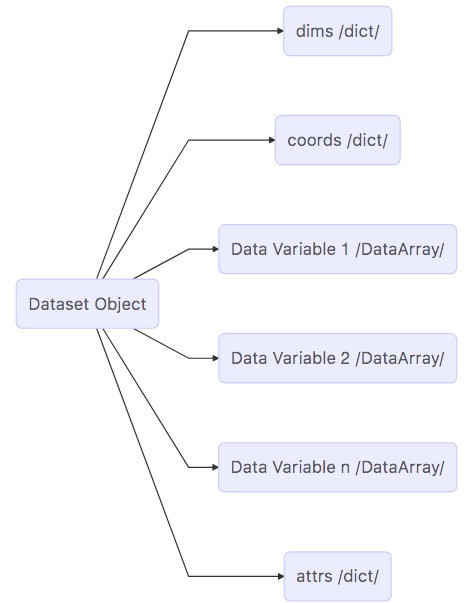
\includegraphics{../figures/Dataset-diagram.png}
\caption{DataArray-diagram}
\end{figure}

    \subsection{The DataArray Object}\label{the-dataarray-object}

It is worth looking at the \texttt{DataArray} object in more detail
because these containers actually store the arrays that we will be using
when analyzing ECCO output. Please see the
\href{http://xarray.pydata.org/en/stable/data-structures.html\#dataarray}{xarray
documentation on the DataArray object} for more information.

\texttt{DataArray} objects are actually very similar to \texttt{Dataset}
objects. Like \texttt{Dataset} objects they also contain dimensions,
coordinates, and attributes. The biggest difference is that they have a
\textbf{name}, a string that identifies the name of the variable, and an
array of \textbf{values}. The \textbf{values} array is a
\href{https://docs.scipy.org/doc/numpy-1.13.0/reference/generated/numpy.array.html}{numpy
array}.

\subsubsection{\texorpdfstring{Examining the \texttt{DataArray\ Object}
contents}{Examining the DataArray Object contents}}\label{examining-the-dataarray-object-contents}

Let's examine the contents of one \texttt{DataArray} found in
\texttt{ds}, \texttt{XC}:

    \begin{Verbatim}[commandchars=\\\{\}]
{\color{incolor}In [{\color{incolor}7}]:} \PY{n}{ds}\PY{o}{.}\PY{n}{XC}
\end{Verbatim}


\begin{Verbatim}[commandchars=\\\{\}]
{\color{outcolor}Out[{\color{outcolor}7}]:} <xarray.DataArray 'XC' (i2: 90, i3: 90)>
        array([[-37.5     , -36.5     , -35.5     , {\ldots},  49.5     ,  50.5     ,  51.5     ],
               [-37.5     , -36.5     , -35.5     , {\ldots},  49.5     ,  50.5     ,  51.5     ],
               [-37.5     , -36.5     , -35.5     , {\ldots},  49.5     ,  50.5     ,  51.5     ],
               {\ldots}, 
               [-37.730072, -37.178291, -36.597565, {\ldots},  50.597565,  51.178291,
                 51.730072],
               [-37.771988, -37.291943, -36.764027, {\ldots},  50.764027,  51.291943,
                 51.771988],
               [-37.837925, -37.44421 , -36.968143, {\ldots},  50.968143,  51.44421 ,
                 51.837925]])
        Coordinates:
          * i2       (i2) float64 1.0 2.0 3.0 4.0 5.0 6.0 7.0 8.0 9.0 10.0 11.0 12.0 {\ldots}
          * i3       (i3) float64 1.0 2.0 3.0 4.0 5.0 6.0 7.0 8.0 9.0 10.0 11.0 12.0 {\ldots}
        Attributes:
            long\_name:  longitude
            units:      degrees\_east
\end{Verbatim}
            
    \subsubsection{\texorpdfstring{Examining the \texttt{DataArray\ Object}
contents}{Examining the DataArray Object contents}}\label{examining-the-dataarray-object-contents}

The layout of the contents of \texttt{DataArray} objects is similar to
those of \texttt{Dataset} objects which makes it easier to understand
the meaning of some of its fields. Let's go through \texttt{ds.XC} piece
by piece, starting from the top.

\paragraph{1. Object type}\label{object-type}

\texttt{\textless{}xarray.DataArray\textgreater{}}

This is indeed a \texttt{DataArray} object from the \texttt{xarray}
package.

\begin{quote}
Note: You can also find the type of an object with the \texttt{type}
command: \texttt{print\ type(ds.XC)}
\end{quote}

    \paragraph{2. Object Name}\label{object-name}

\texttt{XC}

The top line tells us what type of object the variable is. In this case
\texttt{ds} is an instance of the \texttt{Dataset}

\paragraph{3. Dimensions}\label{dimensions}

\texttt{Dimensions:\ \ (i2:\ 90,\ i3:\ 90)}

Unlike the \texttt{ds} object, the XC \texttt{DataArray} only has two
dimensions, \textbf{i2} and \textbf{i3}. This makes sense since the
longitude of the grid cell centers only vary with horizontal location.

\paragraph{4. Array}\label{array}

\begin{verbatim}
array([[-37.5     , -36.5     , -35.5     , ...,  49.5     ,  50.5     ,  51.5     ],
       [-37.5     , -36.5     , -35.5     , ...,  49.5     ,  50.5     ,  51.5     ],
       [-37.5     , -36.5     , -35.5     , ...,  49.5     ,  50.5     ,  51.5     ],
       ..., 
       [-37.730072, -37.178291, -36.597565, ...,  50.597565,  51.178291,
         51.730072],
       [-37.771988, -37.291943, -36.764027, ...,  50.764027,  51.291943,
         51.771988],
       [-37.837925, -37.44421 , -36.968143, ...,  50.968143,  51.44421 ,
         51.837925]])
\end{verbatim}

Unlike the \texttt{Dataset} object there are no
\texttt{Data\ Variables}. Instead, we find an \textbf{array} of values.
Python prints out a subset of the array.

\texttt{DataArray} objects store \emph{only one} array while
\texttt{DataSet} objects store one or more \texttt{DataArrays}.

\paragraph{4. Coordinates}\label{coordinates}

\begin{verbatim}
Coordinates:
  i2       (i2) float64 1.0 2.0 3.0 4.0 5.0 6.0 7.0 8.0 9.0 10.0 11.0 12.0 ...
  i3       (i3) float64 1.0 2.0 3.0 4.0 5.0 6.0 7.0 8.0 9.0 10.0 11.0 12.0 ...
\end{verbatim}

We find two 1D arrays with coordinate labels for \textbf{i2} and
\textbf{i3}.

\paragraph{5. Attributes}\label{attributes}

\begin{verbatim}
Attributes:
    long_name:  longitude
    units:      degrees_east
\end{verbatim}

The \texttt{XC} variable has a \texttt{long\_name} (longitude) and units
(degrees\_east). Of course, this metadata comes from the netCDF file.

    \subsubsection{\texorpdfstring{Accessing the numpy array stored in a
\texttt{DataArray}
object}{Accessing the numpy array stored in a DataArray object}}\label{accessing-the-numpy-array-stored-in-a-dataarray-object}

To access the numpy array storing the values of the variable in the
\texttt{DataArray} object we access its \texttt{values} field as
follows,

    \begin{Verbatim}[commandchars=\\\{\}]
{\color{incolor}In [{\color{incolor}8}]:} \PY{n}{ds}\PY{o}{.}\PY{n}{XC}\PY{o}{.}\PY{n}{values}
\end{Verbatim}


\begin{Verbatim}[commandchars=\\\{\}]
{\color{outcolor}Out[{\color{outcolor}8}]:} array([[-37.5       , -36.5       , -35.5       , {\ldots},  49.5       ,
                 50.5       ,  51.5       ],
               [-37.5       , -36.5       , -35.5       , {\ldots},  49.5       ,
                 50.5       ,  51.5       ],
               [-37.5       , -36.5       , -35.5       , {\ldots},  49.5       ,
                 50.5       ,  51.5       ],
               {\ldots}, 
               [-37.73007202, -37.17829132, -36.5975647 , {\ldots},  50.5975647 ,
                 51.17829132,  51.73007202],
               [-37.77198792, -37.2919426 , -36.76402664, {\ldots},  50.76402664,
                 51.2919426 ,  51.77198792],
               [-37.83792496, -37.44421005, -36.96814346, {\ldots},  50.96814346,
                 51.44421005,  51.83792496]])
\end{Verbatim}
            
    The array that is returned is a numpy n-dimensional array:

    \begin{Verbatim}[commandchars=\\\{\}]
{\color{incolor}In [{\color{incolor}9}]:} \PY{n+nb}{type}\PY{p}{(}\PY{n}{ds}\PY{o}{.}\PY{n}{XC}\PY{o}{.}\PY{n}{values}\PY{p}{)}
\end{Verbatim}


\begin{Verbatim}[commandchars=\\\{\}]
{\color{outcolor}Out[{\color{outcolor}9}]:} numpy.ndarray
\end{Verbatim}
            
    Being a numpy array, one can use all of the numerical operations
provided by the numpy module on it. \textgreater{} ** Note: ** You may
find it useful to learn about the operations that can be made on numpy
arrays. Here is a quickstart guide:
https://docs.scipy.org/doc/numpy-dev/user/quickstart.html

We'll learn more about how to access the values of this array in a later
tutorial. For now it is sufficient to know where to find the arrays!

\subsubsection{\texorpdfstring{Map of the \texttt{DataArray}
Object}{Map of the DataArray Object}}\label{map-of-the-dataarray-object}

Taking another big step back we can now understand the layout of the
\texttt{DataArray} object:

\begin{figure}
\centering
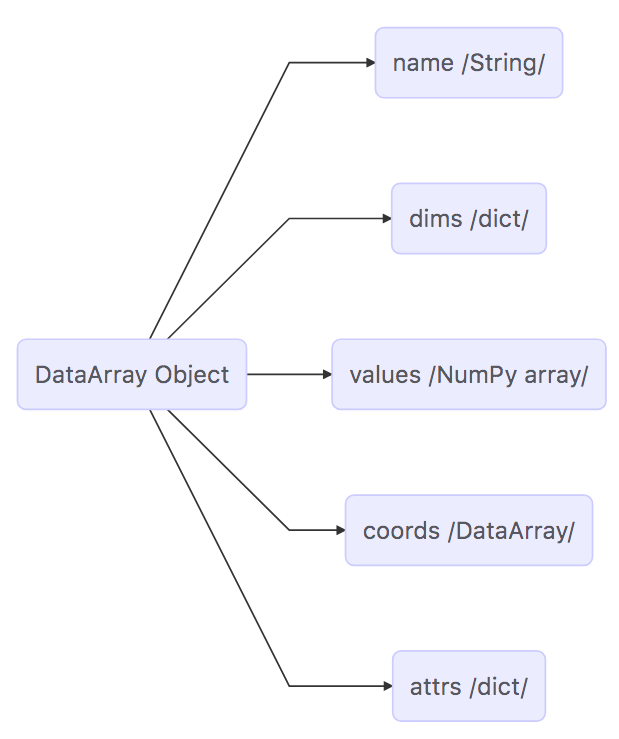
\includegraphics{../figures/DataArray-diagram.png}
\caption{DataArray-diagram}
\end{figure}

    \subsection{Conclusion}\label{conclusion}

Now you know the basics of the \texttt{Dataset} and \texttt{DataArray}
objects that will store the ECCO v4 grid and variables. Now that you're
oriented, go back and take another look at the contents of the grid
\texttt{ds} object that we originally loaded!


    % Add a bibliography block to the postdoc
    
    
    
    \end{document}
